\documentclass[border=8pt]{standalone}
\usepackage{tikz}
\usepackage{tgheros}\renewcommand{\familydefault}{\sfdefault}
\usepackage[T1]{fontenc}
\usepackage{sansmath}
\usetikzlibrary{positioning,fit,backgrounds,calc,arrows.meta}
% ---- reference palette: pale fills + matching mid-tone borders, black text ----
% R2-11a: greyscale for consistency with Figure 1 (colours removed).
\definecolor{txt}{HTML}{000000}
\definecolor{gyF}{HTML}{F2F2F2}\definecolor{gyB}{HTML}{000000}   % light grey fill (AP)
\definecolor{blF}{HTML}{FFFFFF}\definecolor{blB}{HTML}{000000}   % white fill (acquisition, core 0)
\definecolor{gnF}{HTML}{E8E8E8}\definecolor{gnB}{HTML}{000000}   % grey fill (compute, core 1)
\definecolor{rdF}{HTML}{C8C8C8}\definecolor{rdB}{HTML}{000000}   % darker grey fill (output)
\definecolor{socB}{HTML}{000000}
\begin{document}\sansmath
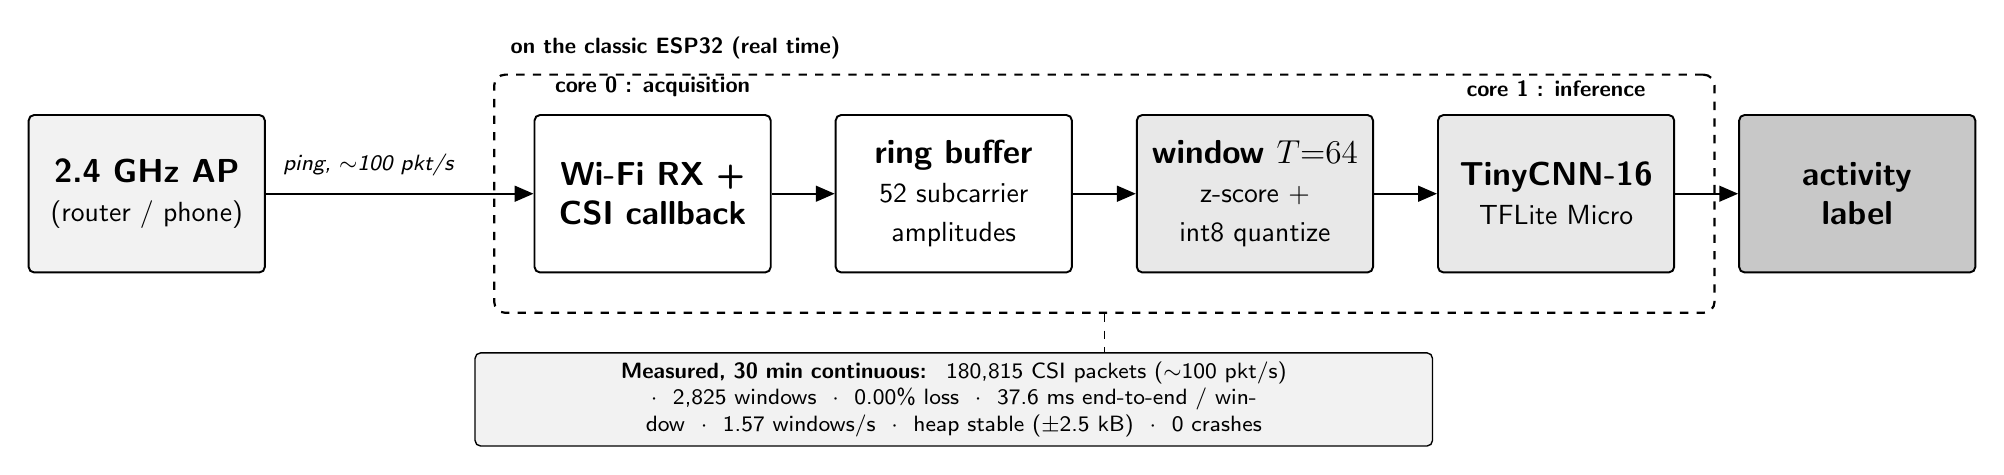
\begin{tikzpicture}[font=\large,text=txt,>={Triangle[length=2.4mm,width=2mm]},node distance=6mm,
  stg/.style={rounded corners=2pt,line width=0.7pt,align=center,inner sep=5pt,minimum height=20mm,minimum width=30mm},
  ap/.style={stg,fill=gyF,draw=gyB},
  acq/.style={stg,fill=blF,draw=blB},
  cmp/.style={stg,fill=gnF,draw=gnB},
  res/.style={stg,fill=rdF,draw=rdB},
  fl/.style={font=\footnotesize\itshape,text=txt},
  core/.style={font=\footnotesize\bfseries,text=socB}]

\node[ap] (ap) {\textbf{2.4 GHz AP}\\\normalsize(router / phone)};
\node[acq,right=34mm of ap] (rx) {\textbf{Wi-Fi RX +}\\\textbf{CSI callback}};
\node[acq,right=8mm of rx] (buf) {\textbf{ring buffer}\\\normalsize 52 subcarrier\\\normalsize amplitudes};
\node[cmp,right=8mm of buf] (win) {\textbf{window $T{=}64$}\\\normalsize z-score +\\\normalsize int8 quantize};
\node[cmp,right=8mm of win] (net) {\textbf{TinyCNN-16}\\\normalsize TFLite Micro};
\node[res,right=8mm of net] (lab) {\textbf{activity}\\\textbf{label}};

\draw[->,line width=0.8pt] (ap) -- (rx);
\node[fl,anchor=south] at ($(ap.east)+(13mm,1mm)$) {ping, $\sim$100 pkt/s};
\draw[->,line width=0.8pt] (rx) -- (buf);
\draw[->,line width=0.8pt] (buf) -- (win);
\draw[->,line width=0.8pt] (win) -- (net);
\draw[->,line width=0.8pt] (net) -- (lab);

% core annotations
\node[core,above=1mm of rx] {core 0 : acquisition};
\node[core,above=1mm of net] {core 1 : inference};

% on-device bracket
\begin{scope}[on background layer]
\node[draw=socB,line width=0.8pt,rounded corners=4pt,dashed,fit=(rx)(buf)(win)(net),inner sep=5mm] (chip) {};
\end{scope}
\node[anchor=south west,font=\footnotesize\bfseries,text=socB] at ([xshift=1mm,yshift=0.6mm]chip.north west) {on the classic ESP32 (real time)};

% measured-metrics band
\node[draw=gyB,fill=gyF,rounded corners=2pt,line width=0.5pt,align=center,
      text width=\dimexpr\linewidth-2mm\relax,below=10mm of buf.south,anchor=north,font=\footnotesize] (band)
  {\textbf{Measured, 30 min continuous:}~ 180{,}815 CSI packets ($\sim$100 pkt/s) ~$\cdot$~ 2{,}825 windows ~$\cdot$~ 0.00\% loss ~$\cdot$~ 37.6 ms end-to-end / window ~$\cdot$~ 1.57 windows/s ~$\cdot$~ heap stable ($\pm$2.5 kB) ~$\cdot$~ 0 crashes};
\draw[gyB,line width=0.5pt,dashed] (chip.south) -- (chip.south|-band.north);

\end{tikzpicture}
\end{document}
